\documentclass[DIV=14,titlepage=false]{scrreprt}

%%%%%%%%%%%%%%%%%%%%%%%%%%%%%%%%%%%%%%%%%%%%%%%%%%%%%%%%%%%%%%%%%%%%%%%%%%%%%%%
%                                Basic Packages                               %
%%%%%%%%%%%%%%%%%%%%%%%%%%%%%%%%%%%%%%%%%%%%%%%%%%%%%%%%%%%%%%%%%%%%%%%%%%%%%%%
% Gives us multiple colors.
\usepackage[usenames,dvipsnames,pdftex]{xcolor}
% Lets us style link colors.
\usepackage{hyperref}
% Lets us import images and graphics.
\usepackage{graphicx}
% Lets us use figures in floating environments.
\usepackage{float}
% Lets us create multiple columns.
\usepackage{multicol}
% Gives us better math syntax.
\usepackage{amsmath,amsfonts,mathtools,amsthm,amssymb}
% Lets us strikethrough text.
\usepackage{cancel}
% Lets us edit the caption of a figure.
\usepackage{caption}
% Lets us import pdf directly in our tex code.
\usepackage{pdfpages}
% Lets us do algorithm stuff.
\usepackage[ruled,vlined,linesnumbered]{algorithm2e}
% Gets rid of some errors.
\usepackage{scrhack}
\def\class{article}
\usepackage{geometry}
\geometry{margin=0.9in}
%%%%%%%%%%%%%%%%%%%%%%%%%%%%%%%%%%%%%%%%%%%%%%%%%%%%%%%%%%%%%%%%%%%%%%%%%%%%%%%
%                                Basic Settings                               %
%%%%%%%%%%%%%%%%%%%%%%%%%%%%%%%%%%%%%%%%%%%%%%%%%%%%%%%%%%%%%%%%%%%%%%%%%%%%%%%

%%%%%%%%%%%%%
%  Symbols  %
%%%%%%%%%%%%%

\let\implies\Rightarrow
\let\impliedby\Leftarrow
\let\iff\Leftrightarrow
\let\epsilon\varepsilon

%%%%%%%%%%%%
%  Tables  %
%%%%%%%%%%%%

\setlength{\tabcolsep}{5pt}
\renewcommand\arraystretch{1.5}

%%%%%%%%%%%%%%%%%%%%%%%
%  Center Title Page  %
%%%%%%%%%%%%%%%%%%%%%%%

\usepackage{titling}
\renewcommand\maketitlehooka{\null\mbox{}\vfill}
\renewcommand\maketitlehookd{\vfill\null}

%%%%%%%%%%%%%%%%%%%%%%%%%%%%%%%%%%%%%%%%%%%%%%%%%%%%%%%
%  Create a grey background in the middle of the PDF  %
%%%%%%%%%%%%%%%%%%%%%%%%%%%%%%%%%%%%%%%%%%%%%%%%%%%%%%%

\usepackage{eso-pic}
\newcommand\definegraybackground{
  \definecolor{reallylightgray}{HTML}{FAFAFA}
  \AddToShipoutPicture{
    \ifthenelse{\isodd{\thepage}}{
      \AtPageLowerLeft{
        \put(\LenToUnit{\dimexpr\paperwidth-222pt},0){
          \color{reallylightgray}\rule{222pt}{297mm}
        }
      }
    }
    {
      \AtPageLowerLeft{
        \color{reallylightgray}\rule{222pt}{297mm}
      }
    }
  }
}

%%%%%%%%%%%%%%%%%%%%%%%%
%  Modify Links Color  %
%%%%%%%%%%%%%%%%%%%%%%%%

\hypersetup{
  % Enable highlighting links.
  colorlinks,
  % Change the color of links to blue.
  linkcolor={black},
  % Change the color of citations to black.
  citecolor={black},
  % Change the color of url's to blue with some black.
  urlcolor=blue
}

%%%%%%%%%%%%%%%%%%
% Fix WrapFigure %
%%%%%%%%%%%%%%%%%%

\newcommand{\wrapfill}{\par\ifnum\value{WF@wrappedlines}>0
    \parskip=0pt
    \addtocounter{WF@wrappedlines}{-1}%
    \null\vspace{\arabic{WF@wrappedlines}\baselineskip}%
    \WFclear
\fi}

%%%%%%%%%%%%%%%%%
% Multi Columns %
%%%%%%%%%%%%%%%%%

\let\multicolmulticols\multicols
\let\endmulticolmulticols\endmulticols

\RenewDocumentEnvironment{multicols}{mO{}}
{%
  \ifnum#1=1
    #2%
  \else % More than 1 column
    \multicolmulticols{#1}[#2]
  \fi
}
{%
  \ifnum#1=1
\else % More than 1 column
  \endmulticolmulticols
\fi
}

\newlength{\thickarrayrulewidth}
\setlength{\thickarrayrulewidth}{5\arrayrulewidth}

%%%%%%%%%%%%%%%%%%%%
%  Import Figures  %
%%%%%%%%%%%%%%%%%%%%

\usepackage{import}
\pdfminorversion=7

% EXAMPLE:
% 1. \incfig{limit-graph}
% 2. \incfig[0.4]{limit-graph}
% Parameters:
% 1. The figure name. It should be located in figures/NAME.tex_pdf.
% 2. (Optional) The width of the figure. Example: 0.5, 0.35.
\newcommand\incfig[2][1]{%
  \def\svgwidth{#1\columnwidth}
  \import{./figures/}{#2.pdf_tex}
}

\begingroup\expandafter\expandafter\expandafter\endgroup
\expandafter\ifx\csname pdfsuppresswarningpagegroup\endcsname\relax
\else
  \pdfsuppresswarningpagegroup=1\relax
\fi

%%%%%%%%%%%%%
%  Correct  %
%%%%%%%%%%%%%

% EXAMPLE:
% 1. \correct{INCORRECT}{CORRECT}
% Parameters:
% 1. The incorrect statement.
% 2. The correct statement.
\definecolor{correct}{HTML}{009900}
\newcommand\correct[2]{{\color{red}{#1 }}\ensuremath{\to}{\color{correct}{ #2}}}



\newcommand{\R}{\mathbb{R}}
\newcommand{\Z}{\mathbb{Z}}
\newcommand{\E}{\mathbb{E}}
\newcommand{\B}{\ensuremath{\mathcal{B}}}
\newcommand{\X}{\ensuremath{\mathcal{X}}}
\newcommand{\Y}{\ensuremath{\mathcal{Y}}}
\newcommand{\mA}{\ensuremath{\mathbf{A}}}
\newcommand{\mB}{\ensuremath{\mathbf{B}}}
\newcommand{\mC}{\ensuremath{\mathbf{C}}}
\newcommand{\mD}{\ensuremath{\mathbf{D}}}
\newcommand{\mX}{\ensuremath{\mathbf{X}}}
\newcommand{\mY}{\ensuremath{\mathbf{Y}}}
\newcommand{\mx}{\ensuremath{\mathbf{x}}}
\newcommand{\my}{\ensuremath{\mathbf{y}}}
\newcommand{\mI}{\ensuremath{\mathbf{I}}}
\newcommand{\mi}{\ensuremath{\mathbf{\iota}}}
\newcommand{\mmu}{\ensuremath{\mathbf{\mu}}}
\newcommand{\mc}{\ensuremath{\mathbf{c}}}
\newcommand{\mSigma}{\ensuremath{\mathbf{\Sigma}}}
\newcommand{\mzero}{\ensuremath{\mathbf{0}}}
\newcommand{\independent}{\perp\!\!\!\!\perp} 
\setlength{\parindent}{0pt}
%%%%%%%%%%%%%%%%%%%%%%%%%%%%%%%%%%%%%%%%%%%%%%%%%%%%%%%%%%%%%%%%%%%%%%%%%%%%%%%
%                                 Environments                                %
%%%%%%%%%%%%%%%%%%%%%%%%%%%%%%%%%%%%%%%%%%%%%%%%%%%%%%%%%%%%%%%%%%%%%%%%%%%%%%%

\usepackage{varwidth}
\usepackage{thmtools}
\usepackage[most,many,breakable]{tcolorbox}

\tcbuselibrary{theorems,skins,hooks}
\usetikzlibrary{arrows,calc,shadows.blur}

%%%%%%%%%%%%%%%%%%%
%  Define Colors  %
%%%%%%%%%%%%%%%%%%%

\definecolor{myblue}{RGB}{45, 111, 177}
\definecolor{mygreen}{RGB}{56, 140, 70}
\definecolor{myred}{RGB}{199, 68, 64}
\definecolor{mypurple}{RGB}{197, 92, 212}

\definecolor{definition}{HTML}{228b22}
\definecolor{theorem}{HTML}{00007B}
\definecolor{example}{HTML}{2A7F7F}
\definecolor{definition}{HTML}{228b22}
\definecolor{prop}{HTML}{191971}
\definecolor{lemma}{HTML}{983b0f}
\definecolor{exercise}{HTML}{88D6D1}

\colorlet{definition}{mygreen!85!black}
\colorlet{claim}{mygreen!85!black}
\colorlet{corollary}{mypurple!85!black}
\colorlet{proof}{theorem}

%%%%%%%%%%%%%%%%%%%%%%
%  Helpful Commands  %
%%%%%%%%%%%%%%%%%%%%%%

% EXAMPLE:
% 1. \createnewtheoremstyle{thmdefinitionbox}{}{}
% 2. \createnewtheoremstyle{thmtheorembox}{}{}
% 3. \createnewtheoremstyle{thmproofbox}{qed=\qedsymbol}{
%       rightline=false, topline=false, bottomline=false
%    }
% Parameters:
% 1. Theorem name.
% 2. Any extra parameters to pass directly to declaretheoremstyle.
% 3. Any extra parameters to pass directly to mdframed.
\newcommand\createnewtheoremstyle[3]{
  \declaretheoremstyle[
  headfont=\bfseries\sffamily, bodyfont=\normalfont, #2,
  mdframed={
    #3,
  },
  ]{#1}
}

% EXAMPLE:
% 1. \createnewcoloredtheoremstyle{thmdefinitionbox}{definition}{}{}
% 2. \createnewcoloredtheoremstyle{thmexamplebox}{example}{}{
%       rightline=true, leftline=true, topline=true, bottomline=true
%     }
% 3. \createnewcoloredtheoremstyle{thmproofbox}{proof}{qed=\qedsymbol}{backgroundcolor=white}
% Parameters:
% 1. Theorem name.
% 2. Color of theorem.
% 3. Any extra parameters to pass directly to declaretheoremstyle.
% 4. Any extra parameters to pass directly to mdframed.
\newcommand\createnewcoloredtheoremstyle[4]{
  \declaretheoremstyle[
  headfont=\bfseries\sffamily\color{#2}, bodyfont=\normalfont, #3,
  mdframed={
    linewidth=2pt,
    rightline=false, leftline=true, topline=false, bottomline=false,
    linecolor=#2, backgroundcolor=#2!5, #4,
  },
  ]{#1}
}

%%%%%%%%%%%%%%%%%%%%%%%%%%%%%%%%%%%
%  Create the Environment Styles  %
%%%%%%%%%%%%%%%%%%%%%%%%%%%%%%%%%%%

\makeatletter
\@ifclasswith\class{nocolor}{
  % Environments without color.

  \createnewtheoremstyle{thmdefinitionbox}{}{}
  \createnewtheoremstyle{thmtheorembox}{}{}
  \createnewtheoremstyle{thmexamplebox}{}{}
  \createnewtheoremstyle{thmclaimbox}{}{}
  \createnewtheoremstyle{thmcorollarybox}{}{}
  \createnewtheoremstyle{thmpropbox}{}{}
  \createnewtheoremstyle{thmlemmabox}{}{}
  \createnewtheoremstyle{thmexercisebox}{}{}
  \createnewtheoremstyle{thmdefinitionbox}{}{}
  \createnewtheoremstyle{thmquestionbox}{}{}
  \createnewtheoremstyle{thmsolutionbox}{}{}

  \createnewtheoremstyle{thmproofbox}{qed=\qedsymbol}{}
  \createnewtheoremstyle{thmexplanationbox}{}{}
}{
  % Environments with color.

  \createnewcoloredtheoremstyle{thmdefinitionbox}{definition}{}{}
  \createnewcoloredtheoremstyle{thmtheorembox}{theorem}{}{}
  \createnewcoloredtheoremstyle{thmexamplebox}{example}{}{
    rightline=true, leftline=true, topline=true, bottomline=true
  }
  \createnewcoloredtheoremstyle{thmclaimbox}{claim}{}{}
  \createnewcoloredtheoremstyle{thmcorollarybox}{corollary}{}{}
  \createnewcoloredtheoremstyle{thmpropbox}{prop}{}{}
  \createnewcoloredtheoremstyle{thmlemmabox}{lemma}{}{}
  \createnewcoloredtheoremstyle{thmexercisebox}{exercise}{}{}

  \createnewcoloredtheoremstyle{thmproofbox}{proof}{qed=\qedsymbol}{backgroundcolor=white}
  \createnewcoloredtheoremstyle{thmexplanationbox}{example}{qed=\qedsymbol}{backgroundcolor=white}
}
\makeatother

%%%%%%%%%%%%%%%%%%%%%%%%%%%%%
%  Create the Environments  %
%%%%%%%%%%%%%%%%%%%%%%%%%%%%%

\declaretheorem[numberwithin=section, style=thmtheorembox,     name=Theorem]{theorem}
\declaretheorem[numbered=no,          style=thmexamplebox,     name=Example]{example}
\declaretheorem[numberwithin=section, style=thmclaimbox,       name=Claim]{claim}
\declaretheorem[numberwithin=section, style=thmcorollarybox,   name=Corollary]{corollary}
\declaretheorem[numberwithin=section, style=thmpropbox,        name=Proposition]{prop}
\declaretheorem[numberwithin=section, style=thmlemmabox,       name=Lemma]{lemma}
\declaretheorem[numberwithin=section, style=thmexercisebox,    name=Exercise]{exercise}
\declaretheorem[numbered=no,          style=thmproofbox,       name=Proof]{replacementproof}
\declaretheorem[numbered=no,          style=thmexplanationbox, name=Proof]{expl}

\makeatletter
\@ifclasswith\class{nocolor}{
  % Environments without color.

  \newtheorem*{note}{Note}

  \declaretheorem[numberwithin=section, style=thmdefinitionbox, name=Definition]{definition}
  \declaretheorem[numberwithin=section, style=thmquestionbox,   name=Question]{question}
  \declaretheorem[numberwithin=section, style=thmsolutionbox,   name=Solution]{solution}
}{
  % Environments with color.

  \newtcbtheorem[number within=section]{Definition}{Definition}{
    enhanced,
    before skip=2mm,
    after skip=2mm,
    colback=red!5,
    colframe=red!80!black,
    colbacktitle=red!75!black,
    boxrule=0.5mm,
    attach boxed title to top left={
      xshift=1cm,
      yshift*=1mm-\tcboxedtitleheight
    },
    varwidth boxed title*=-3cm,
    boxed title style={
      interior engine=empty,
      frame code={
        \path[fill=tcbcolback]
        ([yshift=-1mm,xshift=-1mm]frame.north west)
        arc[start angle=0,end angle=180,radius=1mm]
        ([yshift=-1mm,xshift=1mm]frame.north east)
        arc[start angle=180,end angle=0,radius=1mm];
        \path[left color=tcbcolback!60!black,right color=tcbcolback!60!black,
        middle color=tcbcolback!80!black]
        ([xshift=-2mm]frame.north west) -- ([xshift=2mm]frame.north east)
        [rounded corners=1mm]-- ([xshift=1mm,yshift=-1mm]frame.north east)
        -- (frame.south east) -- (frame.south west)
        -- ([xshift=-1mm,yshift=-1mm]frame.north west)
        [sharp corners]-- cycle;
      },
    },
    fonttitle=\bfseries,
    title={#2},
    #1
  }{def}

  \NewDocumentEnvironment{definition}{O{}O{}}
    {\begin{Definition}{#1}{#2}}{\end{Definition}}

  \newtcolorbox{note}[1][]{%
    enhanced jigsaw,
    colback=gray!20!white,%
    colframe=gray!80!black,
    size=small,
    boxrule=1pt,
    title=\textbf{Note:-},
    halign title=flush center,
    coltitle=black,
    breakable,
    drop shadow=black!50!white,
    attach boxed title to top left={xshift=1cm,yshift=-\tcboxedtitleheight/2,yshifttext=-\tcboxedtitleheight/2},
    minipage boxed title=1.5cm,
    boxed title style={%
      colback=white,
      size=fbox,
      boxrule=1pt,
      boxsep=2pt,
      underlay={%
        \coordinate (dotA) at ($(interior.west) + (-0.5pt,0)$);
        \coordinate (dotB) at ($(interior.east) + (0.5pt,0)$);
        \begin{scope}
          \clip (interior.north west) rectangle ([xshift=3ex]interior.east);
          \filldraw [white, blur shadow={shadow opacity=60, shadow yshift=-.75ex}, rounded corners=2pt] (interior.north west) rectangle (interior.south east);
        \end{scope}
        \begin{scope}[gray!80!black]
          \fill (dotA) circle (2pt);
          \fill (dotB) circle (2pt);
        \end{scope}
      },
    },
    #1,
  }

  \newtcbtheorem{Question}{Question}{enhanced,
    breakable,
    colback=white,
    colframe=myblue!80!black,
    attach boxed title to top left={yshift*=-\tcboxedtitleheight},
    fonttitle=\bfseries,
    title=\textbf{Question:-},
    boxed title size=title,
    boxed title style={%
      sharp corners,
      rounded corners=northwest,
      colback=tcbcolframe,
      boxrule=0pt,
    },
    underlay boxed title={%
      \path[fill=tcbcolframe] (title.south west)--(title.south east)
      to[out=0, in=180] ([xshift=5mm]title.east)--
      (title.center-|frame.east)
      [rounded corners=\kvtcb@arc] |-
      (frame.north) -| cycle;
    },
    #1
  }{def}

  \NewDocumentEnvironment{question}{O{}O{}}
  {\begin{Question}{#1}{#2}}{\end{Question}}

  \newtcolorbox{Solution}{enhanced,
    breakable,
    colback=white,
    colframe=mygreen!80!black,
    attach boxed title to top left={yshift*=-\tcboxedtitleheight},
    title=\textbf{Solution:-},
    boxed title size=title,
    boxed title style={%
      sharp corners,
      rounded corners=northwest,
      colback=tcbcolframe,
      boxrule=0pt,
    },
    underlay boxed title={%
      \path[fill=tcbcolframe] (title.south west)--(title.south east)
      to[out=0, in=180] ([xshift=5mm]title.east)--
      (title.center-|frame.east)
      [rounded corners=\kvtcb@arc] |-
      (frame.north) -| cycle;
    },
  }

  \NewDocumentEnvironment{solution}{O{}O{}}
  {\vspace{-10pt}\begin{Solution}{#1}{#2}}{\end{Solution}}
}
\makeatother

%%%%%%%%%%%%%%%%%%%%%%%%%%%%
%  Edit Proof Environment  %
%%%%%%%%%%%%%%%%%%%%%%%%%%%%

\renewenvironment{proof}[1][\proofname]{\vspace{-10pt}\begin{replacementproof}}{\end{replacementproof}}
\newenvironment{explanation}[1][\proofname]{\vspace{-10pt}\begin{expl}}{\end{expl}}

\theoremstyle{definition}

\newtheorem*{notation}{Notation}
\newtheorem*{previouslyseen}{As previously seen}
\newtheorem*{problem}{Problem}
\newtheorem*{observe}{Observe}
\newtheorem*{property}{Property}
\newtheorem*{intuition}{Intuition}

\setuptoc{toc}{leveldown}

\begin{document}
\vspace{-10pt}
\setcounter{chapter}{16}

\chapter{Panel data. Fixed effects.}
\section{Time invariant heterogeneity}
A panel is a set of observations on individuals, collected over time. An observation is the pair $(y_{it},x_{it})$, where $i$ denotes the individual and $t$ denotes time. The standard panel data specification is that there is an individual-specific effect $\delta_i$ that is constant over time:\[y_{it}=x_{it}\beta+\delta_i+\epsilon_{it}\] such that $\E[\epsilon_{it}|x_{i1},\dots,x_{iT},\delta_i]=0$ (strict exogeneity). If $\delta_i$ is observed then we can estimate $\beta$ by OLS of $y_{it}-\delta_i$ on $x_{it}$. If $\delta_i$  is unobserved then we require either the lack of correlation between $\delta_i$ and $x_{it}$ or the availability of an instrument $w_i$ which is correlated with $x_{it}$ but not $\delta_i+\epsilon_{it}$.\\
\textbf{First differences}\\
If neither of the above are available we can still consistently estimate $\beta$ by considering the regression in first differences:\begin{equation} y_{it}-y_{i,t-1}=(x_{it}-x_{i,t-1})'\beta+(\epsilon_{it}-\epsilon_{i,t-1})\end{equation} which is often written as the regression of $\Delta y_{it}$ on $\Delta x_{it}$, where $\Delta y_{it}=y_{it}-y_{i,t-1}$ and $\Delta x_{it}=x_{it}-x_{i,t-1}$. Running OLS will not be optimal, since there is serial correlation in the error term. Thus the standard errors will be wrong and the estimator inefficient. To solve this we can use GLS.
\section{Within-Group (or simply within) estimator}
Let 
\[
    y_{it}=x_{it}'\beta+\delta_i+\epsilon_{it} \quad \text{where}
\]
\[
    \underset{T\times1}{y_i} = \begin{pmatrix} y_{i1} \\ \vdots \\ y_{iT} \end{pmatrix}, \quad \underset{T\times k}{x_i} = \begin{pmatrix} x_{i1} \\ \vdots \\ x_{iT} \end{pmatrix}, \quad \underset{T\times1}{\epsilon_i} = \begin{pmatrix} \epsilon_{i1} \\ \vdots \\ \epsilon_{iT} \end{pmatrix}
\]
\[
   \underset{nT \times 1}{Y} = \begin{pmatrix} y_{1} \\ \vdots \\ y_{n} \end{pmatrix} =\begin{pmatrix} y_{11} \\ \vdots \\ y_{1T} \\ \vdots \\ y_{n1} \\ \vdots \\ y_{nT} \end{pmatrix}, \quad \underset{nT \times k}{X} = \begin{pmatrix} x_{1} \\ \vdots \\ x_{n} \end{pmatrix}, \quad \underset{nT \times 1}{\epsilon} = \begin{pmatrix} \epsilon_{1} \\ \vdots \\ \epsilon_{n} \end{pmatrix} =\begin{pmatrix} \epsilon_{11} \\ \vdots \\ \epsilon_{1T} \\ \vdots \\ \epsilon_{n1} \\ \vdots \\ \epsilon_{nT} \end{pmatrix}, \quad \underset{n\times1}{\delta} = \begin{pmatrix} \delta_{1} \\ \vdots \\ \delta_{n} \end{pmatrix}
\]
We assume strict exogeneity $\E[\epsilon_i|x_i,\delta_i]=0$ and $Var(\epsilon_i|x_i,\delta_i)=\sigma^2I_T$. We can rewrite equation (1) in terms of the $(T-1)\times T$ matrix D with $D_{tt}=-1,D_{t,t+1}=1$, and all other entries zero: \[ Dy_i = Dx_i \beta + D \delta_i + D \epsilon_i = Dx_i \beta  + D \epsilon_i\]
\begin{align*}
   \underset{(T-1)\times T}{D} =  \begin{pmatrix} -1 & 1 & 0 & \hdots & 0 \\ 0 & -1 & 1 & \ddots & 0\\ \vdots & \ddots & \ddots & \ddots & \vdots \\ 0 & 0 & 0 & -1 & 1 \end{pmatrix} &\implies \underset{(T-1)\times1}{Dy_i} = \begin{pmatrix} y_{i2}-y_{i1} \\ \vdots \\ y_{iT}-y_{i,T-1} \end{pmatrix} = \Delta y_i\\
   &\implies \underset{(T-1)\times k}{Dx_i} = \begin{pmatrix} x_{i2}-x_{i1} \\ \vdots \\ x_{iT}-x_{i,T-1} \end{pmatrix} = \Delta x_i
\end{align*}
This setup can also be written in terms of the matrices $Y,X,\epsilon,\delta$, by considering the block diagonal matrix of D. Our assumptions become $\E[\epsilon|X,\delta]=0$ and $Var(\epsilon|X,\delta)=\sigma^2I_{nT}$. Let $\ell$ be a column vector of ones of length $T$. Then we can write the model as:
\[ Y =X \beta + C \delta + \epsilon \quad \text{where} \quad C = \begin{pmatrix} \ell & 0 & \hdots & 0 \\ 0 & \ell & \hdots & 0 \\ \vdots & \vdots & \ddots & \vdots \\ 0 & 0 & \hdots & \ell \end{pmatrix} \]
\[
\begin{pmatrix}
    D & 0 & \hdots & 0 \\
    0 & D & \hdots & 0 \\
    \vdots & \vdots & \ddots & \vdots \\
    0 & 0 & \hdots & D
\end{pmatrix} Y = \begin{pmatrix}
    D & 0 & \hdots & 0 \\
    0 & D & \hdots & 0 \\
    \vdots & \vdots & \ddots & \vdots \\
    0 & 0 & \hdots & D \end{pmatrix} X \beta
     + \begin{pmatrix}
        D & 0 & \hdots & 0 \\
        0 & D & \hdots & 0 \\
        \vdots & \vdots & \ddots & \vdots \\
        0 & 0 & \hdots & D \end{pmatrix} \epsilon
\]
\begin{note}
\textbf{Definition:} The Kronecker product of two matrices $A$ and $B$, denoted as $A \otimes B$, is a matrix formed by taking each element of $A$ and multiplying it by the entire matrix $B$.

\textbf{Example:} Let $A = \begin{pmatrix} 1 & 2 \\ 3 & 4 \end{pmatrix}$ and $B = \begin{pmatrix} 5 & 6 \\ 7 & 8 \end{pmatrix}$. The Kronecker product $A \otimes B$ is given by:

\[
A \otimes B = \begin{pmatrix} 1 \cdot B & 2 \cdot B \\ 3 \cdot B & 4 \cdot B \end{pmatrix} = \begin{pmatrix} 5 & 6 & 10 & 12 \\ 7 & 8 & 14 & 16 \\ 15 & 18 & 20 & 24 \\ 21 & 24 & 28 & 32 \end{pmatrix}
\]
\textbf{Properties}
\begin{itemize}
    \item  $(A \otimes B)' = A' \otimes B'$
    \item $A\otimes(C + D) = A\otimes C + A\otimes D$
\end{itemize}
There are many other useful properties, but these are all we need for this lecture.
\end{note}
We can now write the first difference estimator more succinctly as:
\[
    (I_n \otimes D)Y = (I_n \otimes D)X \beta + (I_n \otimes D) \epsilon
\]
\textbf{GM Assumptions}
\begin{itemize}
    \item[GM1] rank($I_n \otimes D$)X = k
    \subitem This is equivalent to rank($D$)X = k, which is equivalent to rank($X$) = k
    \item[GM2] $\E[\Delta \epsilon | \Delta X] = 0$
    \subitem $\E[(I_n \otimes D) \epsilon | \Delta X] = (I_n \otimes D)\E[\epsilon|\Delta X] = 0$
    \item[GM3] Homoskedasticity and no serial correlation in $\Delta \epsilon$
    \subitem Even if we assume that $\epsilon_{it}$ is homoskedastic and serially uncorrelated, $\Delta \epsilon_{it}$ will not be. $Cov(\epsilon_{it}-\epsilon_{i,t-1},\epsilon_{i,t-1}-\epsilon_{i,t-2}) = -Var(\epsilon_{it}|x_i) = -\sigma^2 \not = 0$.
\end{itemize}
Since GM1 and GM2 hold, the FD below is unbiased and consistent. 
\[
    \hat\beta_{FD} = \left(\sum_{i=1}^n (Dx_i)'(Dx_i)\right)^{-1} \left(\sum_{i=1}^n (Dx_i)'(Dy_i)\right)
\]
However GM3 is violated so the OLS estimate is not BLUE. To get the efficient estimator we need to use GLS.
\begin{definition}[GLS]
    If instead of GM3 we have that $Var(\epsilon|X) = \Omega$ where $\Omega$ is known, then we can transform the data by premultiplying by $\Omega^{-1/2}$ to get: $Y^* = \Omega^{-1/2}Y, X^* = \Omega^{-1/2}X, \epsilon^* = \Omega^{-1/2}\epsilon$. Then we can run OLS on $Y^* = X^* \beta + \epsilon^*$ to get the efficient estimator $\hat\beta_{GLS} = (X'\Omega^{-1}X)^{-1}X'\Omega^{-1}Y$.\\
    Note that $\Omega$ can be scaled without any effect on the estimator.
\end{definition}
We can see this results in efficient estimates by considering $Var(\epsilon^*|X^*) = \Omega^{-1/2}Var(\epsilon|X)\Omega^{-1/2} =\Omega^{-1/2}\Omega \Omega^{-1/2}= I_{nT}$. We now derive the GLS estimator for the FD model. We assume that the original regression satisfies $\E[\epsilon|X]=0$ and $Var(\epsilon|X)=\sigma^2 I_{nT}$. Then,
\begin{align*}
    Var ((I_n \otimes D)\epsilon|X) &= (In \otimes D) Var(\epsilon|X) (In \otimes D)' \\
    &= \sigma^2 \begin{pmatrix}
        D & 0 & \hdots & 0 \\
        0 & D & \hdots & 0 \\
        \vdots & \vdots & \ddots & \vdots \\
        0 & 0 & \hdots & D  \end{pmatrix} 
        \begin{pmatrix}
            D' & 0 & \hdots & 0 \\
            0 & D' & \hdots & 0 \\
            \vdots & \vdots & \ddots & \vdots \\
            0 & 0 & \hdots & D'  \end{pmatrix} \\
    &= \sigma^2 \begin{pmatrix}
        DD' & 0 & \hdots & 0 \\
        0 & DD' & \hdots & 0 \\
        \vdots & \vdots & \ddots & \vdots \\
        0 & 0 & \hdots & DD'  \end{pmatrix} 
\end{align*}
We thus have our covariance matrix to use for scaling,
\[
    \Omega = \sigma^2 \begin{pmatrix}
        DD' & 0 & \hdots & 0 \\
        0 & DD' & \hdots & 0 \\
        \vdots & \vdots & \ddots & \vdots \\
        0 & 0 & \hdots & DD'  \end{pmatrix}
    \implies \Omega^{-1/2} = \frac{1}{\sigma}\begin{pmatrix}
        (DD')^{-1/2} & 0 & \hdots & 0 \\
        0 & (DD')^{-1/2} & \hdots & 0 \\
        \vdots & \vdots & \ddots & \vdots \\
        0 & 0 & \hdots & (DD')^{-1/2}  \end{pmatrix} 
\]
Thus,
\begin{align*}
    \hat \beta_{GLS-FD} &= \left(((I_n \otimes D)X)'\Omega^{-1}(I_n \otimes D)X\right)^{-1}((I_n \otimes D)X)'\Omega^{-1}(I_n \otimes D)Y \\
    &= \left(X'(I_n \otimes D)' (I_n \otimes (DD')^{-1}) (I_n \otimes D)X\right)^{-1}X'(I_n \otimes D)'(I_n \otimes (DD')^{-1}) (I_n \otimes D)Y \\
    &=\left(X'(I_n \otimes D') (I_n \otimes (DD')^{-1}) (I_n \otimes D)X\right)^{-1}X'(I_n \otimes D')(I_n \otimes (DD')^{-1}) (I_n \otimes D)Y \\
    &=\left(X'(I_n \otimes D'(DD')^{-1}D)X\right)^{-1}X'(I_n \otimes D'(DD')^{-1}D)Y 
\end{align*}
Note that $D'(DD')^{-1}D$  is a projection matrix onto the space spanned by columns of D' (and thus is symmetric and idempotent). We now consider the column vector of 1s $\ell$. Since the FD of $\ell$ is zero (i.e. always $1-1$), we have that $D'\ell = 0$. Thus a projection onto the space spanned by $D'$ is equivalent to projection onto the space orthogonal to $\ell$.
\[ \implies D'(DD')^{-1}D = I_T - \ell(\ell'\ell)^{-1}\ell' = \frac{1}{T}\ell\ell'\]
Then,
\begin{align*}
    \hat \beta_{GLS-FD} &= \left(X'(I_n \otimes (I_T - \frac{1}{T}\ell\ell'))X\right)^{-1}X'(I_n \otimes (I_T - \frac{1}{T}\ell\ell'))Y \\
    &=\left(\sum_{i=1}^{n}x_i'(I_T - \frac{1}{T}\ell\ell')x_i\right)^{-1} \left(\sum_{i=1}^{n}x_i'(I_T - \frac{1}{T}\ell\ell')y_i\right)\\
    &= \left(\sum_{i=1}^{n}x_i'(x_i - \ell\frac{\ell'x_i}{T})\right)^{-1} \left(\sum_{i=1}^{n}x_i'(y_i - \ell\frac{\ell'y_i}{T})\right)
\end{align*}
\[x_i - \ell\frac{\ell'x_i}{T} = \begin{pmatrix}
    x_{i1} \\
    \vdots \\
    x_{iT}
\end{pmatrix}
- \frac{1}{T}\begin{pmatrix}
    \ell'x_i \\
    \vdots \\
    \ell'x_i 
\end{pmatrix}
= \begin{pmatrix}
    x_{i1} - \frac{1}{T}\sum_{t=1}^{T}x_{it} \\
    \vdots \\
    x_{iT} - \frac{1}{T}\sum_{t=1}^{T}x_{it}
\end{pmatrix} = \underbrace{\begin{pmatrix}
    x_{i1} - \bar x_i \\
    \vdots \\
    x_{iT} - \bar x_i
\end{pmatrix}}_{T \times k}
\]
\begin{align*}
    \hat \beta_{GLS-FD} &=\left(\sum_{i=1}^{n}x_i'(x_i -\bar x_i)\right)^{-1} \left(\sum_{i=1}^{n}x_i'(y_i - \bar y_i)\right) \\
    &= \left(\sum_{i=1}^{n}\sum_{t=1}^{T}(x_{it} -\bar x_i)(x_{it} -\bar x_i)'\right)^{-1} \left(\sum_{i=1}^{n}\sum_{t=1}^{T}(x_{it} -\bar x_i)(y_{it} - \bar y_i)\right) 
\end{align*}
This estimator is known as the within or within-group estimator because it exploits only the variation of $x_{it}$ and $y_{it}$ within the groups of observations corresponding to the same individual but different time periods. It ignores the variability between groups by subtracting individual specific time averages from the data. Note that the errors are not uncorrelated, indeed every error term appears in every other equation (via the demeaning).\\

\begin{minipage}[c]{0.5\textwidth} 
    A geometric interpretation of the within transformation is given here. The individual effects are the 'intercepts' of the individual specific scatters. Here they are negatively correlated with $x_it$ so fitting that regression line to the untransformed data results in negative bias. The within transformation shifts the data so that the individual specific scatters have zero intercepts, and thus the regression line is unbiased.
\end{minipage}
\hfill
\begin{minipage}[c]{0.45\textwidth}
    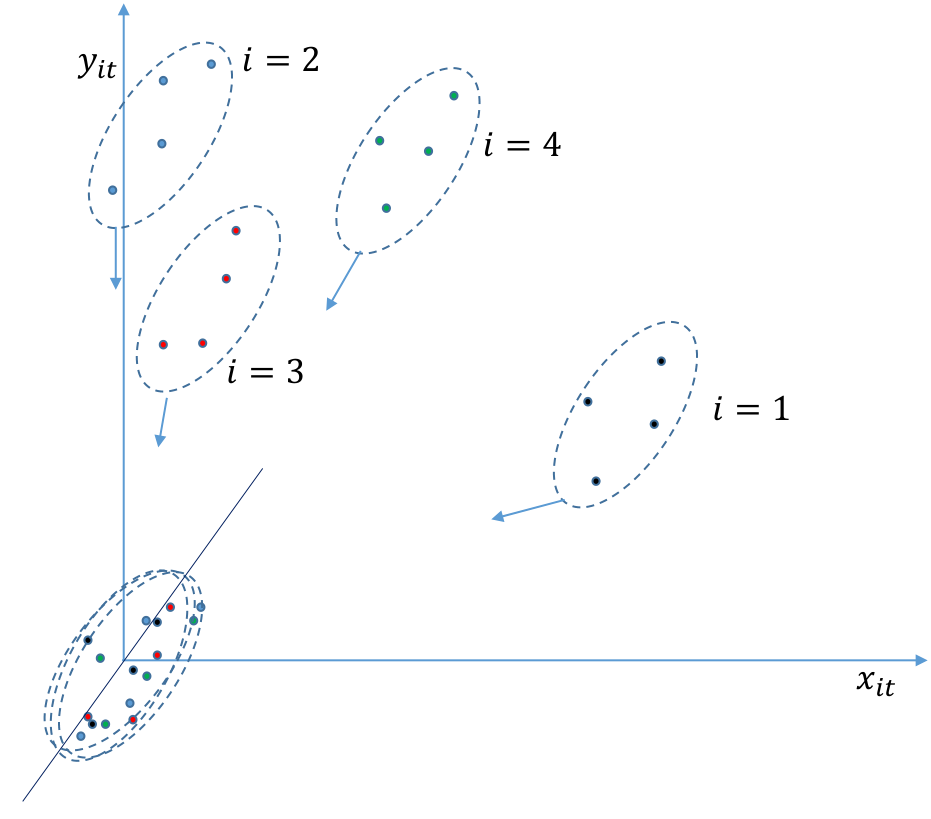
\includegraphics[width=\textwidth]{./Images/fixedeffects.png}
\end{minipage}

\textbf{END OF LECTURE}
\end{document}